\section{$k^2$-Trees}

\begin{Definition}
  The \defi{$k^2$-tree}{$k^2$-Tree} is a datastructure that partitions an $s \times s$-grid into $k^2$ equal sized quadrants. This partition is represented as the root of a $k^2$-ary cardinal tree. The decomposition is done recursively on each subgrid until it has size $1 \times 1$.
\end{Definition}

For $k = 2$ the $k^2$-tree is also known as a \defi{quadtree}{Quadtree}. In the following examples we will always choose $k = 2$ for simplicity.

We will use $k^2$-trees to answer (weighted) two-dimensional range queries on a grid. Given a rectangular region $[x_1, x_2] \times [y_1, y_2]$, count/report the (top-$l$) points in it. A $k^2$-tree cannot count the points without traversing them all, so we will only consider report queries.

Although we cannot prove a good runtime for the $k^2$-tree or -treap, both perform quite well in practice.

\subsection{Unweighted Points}
To report all points in the given range $[x_1, x_2] \times [y_1, y_2]$ we traverse the $k^2$-tree. Starting with the root, at each node we check whether its child ranges (at least partially) overlap with the query range. If so, we step down into these children until ending at a leaf reporting its value. If a child does not overlap the query range, we do not step down into it. This is again shown in Algorithm~\ref{alg:k2TreeReport}.

\begin{algorithm}[htb]
  \begin{codebox}
    \Procname{$\proc{Report}([x_1, x_2] \times [y_1, y_2])$}
    \li $\proc{Report-Recursive}(\attrib{K}{root}, [x_1, x_2] \times [y_1, y_2])$
  \end{codebox}
  \vspace{1mm}
  \begin{codebox}
    \Procname{$\proc{Report-Recursive}(v, [x_1, x_2] \times [y_1, y_2])$}
    \li \If $s \isequal 1$
        \Then
    \li   \textbf{output} $v$
    \li \Else
    \li   \For \textbf{each} child $w$ of $v$
          \Do
    \li     \If \attrib{w}{range} intersects $[x_1, x_2] \times [y_1, y_2]$
            \Then
    \li       $\proc{Report-Recursive}(w, [x_1, x_2] \times [y_1, y_2])$
            \End
          \End
        \End
  \end{codebox}
  \caption{Reports the points from $k^2$-tree $T$ in range $[x_1, x_2] \times [y_1, y_2]$.}
  \label{alg:k2TreeReport}
\end{algorithm}

\subsection{Weighted Points}
To handle weighted points, we annotate each node of the $k^2$-tree with the position and weight of the heaviest element in its corresponding subgrid (ties are broken arbitrarily). Then this element is removed from the grid, so that the children contain the next smaller maximal values of their corresponding subgrid. This gives the tree an additional max-heap structure, it is therefore also known as a \defi{$k^2$-treap}{$k^2$-Treap}.

\begin{Example}
  Consider the $8 \times 8$-grid shown in Figure~\ref{fig:k2TreapGrid}. The corresponding $2^2$-treap is shown in Figure~\ref{fig:k2Treap}. The root is annotated with $(3, 0) : 8$, meaning that the maximal value is $8$ and is in the cell at coordinates $(3, 0)$ of the grid. Because it is then deleted, the maximum in the subgrid $[3, 4] \times [0, 1]$ is $2$ (the only remaining value in this subgrid).

  \begin{figure}[htb]
    \centering
    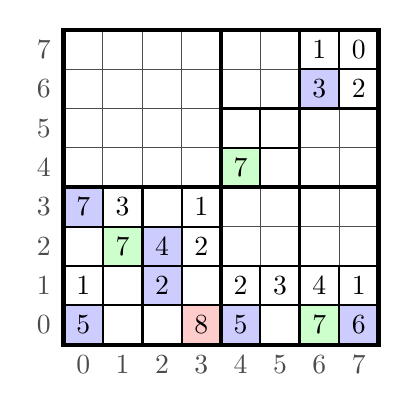
\begin{tikzpicture}[x={(5mm, 0mm)}, y={(0mm, 5mm)}]
  \fill[red!20!white] (3, 0) -- (4, 0) -- (4, 1) -- (3, 1) -- cycle;
  \fill[green!20!white] (1, 2) -- (2, 2) -- (2, 3) -- (1, 3) -- cycle;
  \fill[green!20!white] (6, 0) -- (7, 0) -- (7, 1) -- (6, 1) -- cycle;
  \fill[green!20!white] (4, 4) -- (5, 4) -- (5, 5) -- (4, 5) -- cycle;
  \fill[blue!20!white] (0, 0) -- (1, 0) -- (1, 1) -- (0, 1) -- cycle;
  \fill[blue!20!white] (2, 1) -- (3, 1) -- (3, 2) -- (2, 2) -- cycle;
  \fill[blue!20!white] (0, 3) -- (1, 3) -- (1, 4) -- (0, 4) -- cycle;
  \fill[blue!20!white] (2, 2) -- (3, 2) -- (3, 3) -- (2, 3) -- cycle;
  \fill[blue!20!white] (4, 0) -- (5, 0) -- (5, 1) -- (4, 1) -- cycle;
  \fill[blue!20!white] (7, 0) -- (8, 0) -- (8, 1) -- (7, 1) -- cycle;
  \fill[blue!20!white] (6, 6) -- (7, 6) -- (7, 7) -- (6, 7) -- cycle;

  \foreach \d in {0, 1, ..., 8} {
    \draw[black!70!white] (\d, 0) to (\d, 8);
    \draw[black!70!white] (0, \d) to (8, \d);
  }
  \foreach \d in {0, 1, ..., 7} {
    \node[black!70!white] (c\d) at (\d + 0.5, -0.5) {$\d$};
    \node[black!70!white] (l\d) at (-0.5, \d + 0.5) {$\d$};
  }
  \draw[line width=1.5pt] (0, 0) to (0, 8) to (8, 8) to (8, 0) to (0, 0) to (0, 8);
  \draw[line width=1.5pt] (0, 4) to (8, 4);
  \draw[line width=1.5pt] (4, 0) to (4, 8);
  \draw[line width=1pt] (0, 2) to (8, 2);
  \draw[line width=1pt] (2, 0) to (2, 4);
  \draw[line width=1pt] (6, 0) to (6, 8);
  \draw[line width=1pt] (4, 6) to (8, 6);
  \draw[line width=0.7pt] (1, 0) to (1, 4);
  \draw[line width=0.7pt] (3, 0) to (3, 4);
  \draw[line width=0.7pt] (5, 0) to (5, 2);
  \draw[line width=0.7pt] (7, 0) to (7, 2);
  \draw[line width=0.7pt] (5, 4) to (5, 6);
  \draw[line width=0.7pt] (7, 6) to (7, 8);
  \draw[line width=0.7pt] (0, 1) to (8, 1);
  \draw[line width=0.7pt] (0, 3) to (4, 3);
  \draw[line width=0.7pt] (4, 5) to (6, 5);
  \draw[line width=0.7pt] (6, 7) to (8, 7);

  \foreach \d/\x/\y in {5/0/0, 8/3/0, 5/4/0, 7/6/0, 6/7/0,
                        1/0/1, 2/2/1, 2/4/1, 3/5/1, 4/6/1, 1/7/1,
                        7/1/2, 4/2/2, 2/3/2,
                        7/0/3, 3/1/3, 1/3/3,
                        7/4/4,
                        3/6/6, 2/7/6,
                        1/6/7, 0/7/7} {
    \node (\d\x\y) at (\x + 0.5, \y + 0.5) {$\d$};
  }
\end{tikzpicture}

    \caption{An $8 \times 8$ grid with weights in some cells. The thick lines show the subdivision for a $2^2$-treap. The red cell is the overall maximum. After deleting it, the green cells are maximal in their corresponding $4 \times 4$ grid. After deleting them as well, the blue cells are maximal in their corresponding $2 \times 2$ grids.}
    \label{fig:k2TreapGrid}
  \end{figure}


  \begin{figure}[htb]
    \centering
    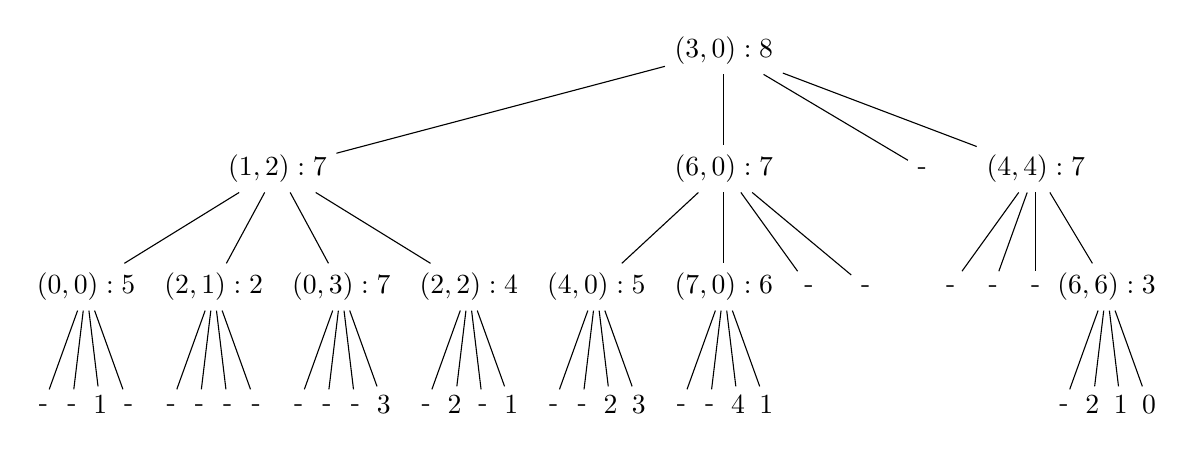
\begin{tikzpicture}[x = {(1.8mm, 0mm)}, y={(0mm, -15mm)}]
  \node (v1) at (18, 0) {$(3, 0) : 8$};

  \node (v2) at (-13.5, 1) {$(1, 2) : 7$};
  \draw (v1) -- (v2);
  
  \node (v3) at (18, 1) {$(6, 0) : 7$};
  \draw (v1) -- (v3);

  \node (v4) at (32, 1) {-};
  \draw (v1) -- (v4);

  \node (v5) at (40, 1) {$(4, 4) : 7$};
  \draw (v1) -- (v5);

  \node (v6) at (-27, 2) {$(0, 0) : 5$};
  \draw (v2) -- (v6);

  \node (v7) at (-18, 2) {$(2, 1) : 2$};
  \draw (v2) -- (v7);

  \node (v8) at (-9, 2) {$(0, 3) : 7$};
  \draw (v2) -- (v8);

  \node (v9) at (0, 2) {$(2, 2) : 4$};
  \draw (v2) -- (v9);

  \node (v10) at (-30, 3) {-};
  \draw (v6) -- (v10);

  \node (v11) at (-28, 3) {-};
  \draw (v6) -- (v11);

  \node (v12) at (-26, 3) {$1$};
  \draw (v6) -- (v12);

  \node (v13) at (-24, 3) {-};
  \draw (v6) -- (v13);

  \node (v14) at (-21, 3) {-};
  \draw (v7) -- (v14);

  \node (v15) at (-19, 3) {-};
  \draw (v7) -- (v15);

  \node (v16) at (-17, 3) {-};
  \draw (v7) -- (v16);

  \node (v17) at (-15, 3) {-};
  \draw (v7) -- (v17);

  \node (v18) at (-12, 3) {-};
  \draw (v8) -- (v18);

  \node (v19) at (-10, 3) {-};
  \draw (v8) -- (v19);

  \node (v20) at (-8, 3) {-};
  \draw (v8) -- (v20);

  \node (v21) at (-6, 3) {$3$};
  \draw (v8) -- (v21);

  \node (v22) at (-3, 3) {-};
  \draw (v9) -- (v22);

  \node (v23) at (-1, 3) {$2$};
  \draw (v9) -- (v23);

  \node (v24) at (1, 3) {-};
  \draw (v9) -- (v24);

  \node (v25) at (3, 3) {$1$};
  \draw (v9) -- (v25);

  \node (v26) at (9, 2) {$(4, 0) : 5$};
  \draw (v3) -- (v26);

  \node (v27) at (18, 2) {$(7, 0) : 6$};
  \draw (v3) -- (v27);

  \node (v28) at (24, 2) {-};
  \draw (v3) -- (v28);

  \node (v29) at (28, 2) {-};
  \draw (v3) -- (v29);

  \node (v30) at (6, 3) {-};
  \draw (v26) -- (v30);

  \node (v31) at (8, 3) {-};
  \draw (v26) -- (v31);

  \node (v32) at (10, 3) {$2$};
  \draw (v26) -- (v32);

  \node (v33) at (12, 3) {$3$};
  \draw (v26) -- (v33);

  \node (v34) at (15, 3) {-};
  \draw (v27) -- (v34);

  \node (v35) at (17, 3) {-};
  \draw (v27) -- (v35);

  \node (v36) at (19, 3) {$4$};
  \draw (v27) -- (v36);

  \node (v37) at (21, 3) {$1$};
  \draw (v27) -- (v37);

  \node (v38) at (34, 2) {-};
  \draw (v5) -- (v38);

  \node (v39) at (37, 2) {-};
  \draw (v5) -- (v39);

  \node (v40) at (40, 2) {-};
  \draw (v5) -- (v40);

  \node (v41) at (45, 2) {$(6, 6) : 3$};
  \draw (v5) -- (v41);

  \node (v42) at (42, 3) {-};
  \draw (v41) -- (v42);

  \node (v43) at (44, 3) {$2$};
  \draw (v41) -- (v43);

  \node (v44) at (46, 3) {$1$};
  \draw (v41) -- (v44);

  \node (v45) at (48, 3) {$0$};
  \draw (v41) -- (v45);
\end{tikzpicture}

    \caption{The $2^2$-treap for the grid shown in Figure~\ref{fig:k2TreapGrid}. The notation of the vertices shows first the position of the maximal element in the corresponding subgrid and then its value. The position is omitted on the last layer, since the corresponding subgrid has size $1 \times 1$.}
    \label{fig:k2Treap}
  \end{figure}
\end{Example}

To extract the heaviest points we use a max-priority-queue~\id{PQ}. Initially we insert the root of the $k^2$-treap. Whenever we pop a vertex from~\id{PQ}, we add all its non-empty children that intersect the query range into it. If the maximal element stored at the current vertex is inside the range, we add it to our result. Otherwise we ignore it and continue with the next node in the priority-queue. The pseudocode is given in Algorithm~\ref{alg:k2TreapReport}.

\begin{algorithm}[htb]
  \begin{codebox}
    \Procname{$\proc{Report}(x_1, x_2, y_1, y_2, l)$}
    \li $\id{PQ} \gets$ empty max-priority-queue
    \li $r \gets \attrib{T}{root}$
    \li $\attribii{PQ}{insert}(r)$ \>\>\>\>\Comment Priority-queue ordered by weight annotated to each vertex.
    \li $c \gets 0$
    \li \While not $\attribii{PQ}{empty}()$ and $c < l$
        \Do
    \li   $v \gets \attribii{PQ}{top}()$
    \li   $\attribii{PQ}{pop}()$
    \li   \If $x_1 \leq \attrib{v}{x} \leq x_2$ and $y_1 \leq \attrib{v}{y} \leq y_2$
          \Then
    \li     \textbf{output} $v$
    \li     $c \gets c + 1$
          \End
    \li   \For \textbf{each} child $w$ of $v$
          \Do
    \li     \If \attrib{w}{range} intersects $[x_1, x_2] \times [y_1, y_2]$
            \Then
    \li       $\attribii{PQ}{push}(w)$
            \End
          \End
        \End
  \end{codebox}
  \caption{Reports the top-$l$ points from $k^2$-treap $T$ in $[x_1, x_2] \times [y_1, y_2]$.}
  \label{alg:k2TreapReport}
\end{algorithm}
